\documentclass[../../main.tex]{subfiles}

\begin{document}
\chapter{Generazione di WebAssembly}
La ricerca di soluzioni efficienti e portabili per eseguire codice in ambienti diversi è diventata una priorità fondamentale nell'informatica moderna. In questo contesto, WebAssembly (Wasm) emerge come una tecnologia chiave, fornendo un formato binario sicuro, veloce e indipendente dalla piattaforma. Nel corso di questo capitolo, esploriamo il processo di generazione di codice WebAssembly attraverso un compilatore dedicato a un linguaggio personalizzato.
Il nostro linguaggio, creato per soddisfare specifiche esigenze o paradigmi di programmazione unici, si propone di offrire una flessibilità senza precedenti agli sviluppatori. Attraverso un compilatore appositamente progettato, saremo in grado di tradurre il codice sorgente del nostro linguaggio in istruzioni Wasm, consentendo così l'esecuzione di programmi in un ambiente virtuale altamente performante e sicuro.
Nel corso di questo capitolo, esamineremo in dettaglio il processo di compilazione, passando attraverso le fasi cruciali che trasformano il nostro codice sorgente in un modulo WebAssembly. Dalla rappresentazione intermedia alla gestione delle dipendenze, esploreremo come il compilatore si adatta alle specificità del nostro linguaggio per garantire una corretta esecuzione e ottimizzazione delle risorse.
Il capitolo si propone inoltre di approfondire le sfide e le opportunità che emergono durante il processo di generazione di WebAssembly. Analizzeremo le scelte di progettazione del compilatore, l'ottimizzazione del codice e la gestione delle risorse, fornendo un quadro completo delle considerazioni che guidano il nostro approccio alla generazione di codice Wasm.

\section{Introduzione WebAssembly}
WebAssembly (Wasm) è un formato di istruzioni altamente performante, portabile e sicuro, progettato per essere eseguito in ambienti virtuali. Originariamente concepito da un gruppo di lavoro congiunto tra Google, Mozilla, Microsoft e Apple, il principale obiettivo di WebAssembly è fornire un formato binario indipendente dalla piattaforma, garantendo al contempo sicurezza e velocità. Sebbene sia stato ideato principalmente per essere eseguito all'interno dei browser web, Wasm trova applicazioni anche in contesti diversi come server, dispositivi IoT e applicazioni desktop.

Le istruzioni Wasm si distinguono dalle istruzioni di un processore reale in quanto sono progettate per l'esecuzione in un ambiente virtuale. Ciò implica che le istruzioni Wasm non possono essere eseguite direttamente da un processore fisico; richiedono invece una traduzione preliminare in istruzioni native. Questo processo di traduzione è gestito da un motore di runtime, il quale interpreta le istruzioni Wasm e le traduce in istruzioni native del sistema ospite. Oltre alla traduzione delle istruzioni, il motore di runtime si occupa anche della gestione della memoria e delle risorse del sistema, fornendo un'astrazione sicura e indipendente dalla piattaforma.

In sintesi, WebAssembly rappresenta una tecnologia versatile e potente che offre un'alternativa efficace alle tradizionali soluzioni di esecuzione di codice, consentendo l'esecuzione di applicazioni web e non solo in modo efficiente, sicuro e indipendente dalla piattaforma di destinazione.\cite{WebAssemblyDoc}

\section{WebAssembly Text Format}
Il formato di testo WebAssembly (WAT) \cite{WebAssemblyTextFormat} è un formato di testo leggibile dall'uomo per la rappresentazione di moduli WebAssembly. Il formato è stato progettato per essere utilizzato come rappresentazione intermedia durante il processo di compilazione, fornendo un'astrazione leggibile dall'uomo per il codice Wasm.
Il compilatore che abbiamo sviluppato generiamo un file .wat ed in seguito il tool wat2wasm \cite{jain2022webassembly} genera il file .wasm, che a sua volta potrá essere eseguito da un motore di runtime.

I tipi di dati che troviamo in wat sono:
\begin{itemize}
    \item \textbf{i32} 32-bit integer
    \item \textbf{i64} 64-bit integer
    \item \textbf{f32} 32-bit float
    \item \textbf{f64} 64-bit float
\end{itemize}
Un singolo  parametro \textit{(param i32)} e il tipo di ritorno \textit{(result i32)}.
\begin{lstlisting}[language=WebAssembly, caption={Esempio di funzione in wat}, label={lst:funzioneWat}]
    (func (param i32) (param i32) (result f64) ...)
\end{lstlisting}
I parametri locali possono essere dichiarati all'interno di una funzione, e sono accessibili solo all'interno della funzione stessa.
I comandi \textit{local.get} e \textit{local.set} vengono utilizzati per accedere agli indici dei parametri locali.
Possiamo usare anche l'operatore \$ per accedere ai parametri locali, in maniera più human-readable.
\begin{lstlisting}[language=WebAssembly, caption={Esempio di funzione in wat}, label={lst:funzioneWat}]
    (func $fun (param i32) (param i32) (result f64)
        (local $par1 i32)
        (local $par2 i32)
        (local $par3 f64)
        ...
        (local.get $par1)
        (local.get $par2)
        (local.set $par3)
        ...
    )
\end{lstlisting}
Come vediamo in questo esempio la funzione \$fun prende in input due parametri di tipo intero e ritorna un valore di tipo float. Inoltre all'interno della funzione vengono dichiarati tre parametri locali, due di tipo intero e uno di tipo float.

\subsubsection{Stack Machine}
L'esecuzione del WebAssembly é definita in termini di Stack-Machine, dove l'idea generale é che ogni tipo di istruzione esegue operazioni di tipo \textit{push/pop} dallo stack.
Quando viene chiamata una funzione, inizia con uno stack vuoto che viene gradualmente riempito e svuotato man mano che le istruzioni del corpo vengono eseguite. Quindi, ad esempio, dopo aver eseguito la seguente funzione:
\begin{lstlisting}[language=WebAssembly]
    (func $somma(param $p1 i32)(param $p2 i32)
        (result i32)
        local.get $p1
        local.get $p2
        i32.add)
\end{lstlisting}
Quando viene chiamata la funzione \$somma, viene passato il precedente valore nella pila come parametro \$p1. La prima istruzione \textit{local.get} copia il valore di \$p1 nello stack, e la seconda istruzione \textit{local.get} copia il valore di \$p2 nello stack. Infine, l'istruzione \textit{i32.add} rimuove i due valori superiori dello stack, li somma e inserisce il risultato nello stack. Alla fine dell'esecuzione della funzione, lo stack contiene il risultato della somma dei due valori passati come parametro.
Per eseguire la \textbf{chiamata della funzione} precedente, vediamo il codice seguente:
\begin{lstlisting}[language=WebAssembly]
    (func $main
        (result i32)
        i32.const 10
        i32.const 5
        call $somma)
\end{lstlisting}
La prima istruzione \textit{i32.const} inserisce il valore constante 10 nello stack, e la seconda istruzione \textit{call} chiama la funzione \$somma. La funzione \$somma viene eseguita, e il risultato viene inserito nello stack. Alla fine dell'esecuzione della funzione, lo stack contiene il risultato della somma dei due valori passati come parametro.
Dobbiamo inoltre aggiungere una dichiarazione di esportazione per fare in modo che la funzione sia visibile all'esterno del modulo(per esempio anche dal codice javascript).
\begin{lstlisting}[language=WebAssembly]
    (export "main"(func $main))
\end{lstlisting}
La prima stringa ``main'' é il nome della funzione che vogliamo esportare e che sara visibile anche all'esterno del modulo, mentre la seconda é l'identificativo della funzione a cui fa riferimento.

\section{CostCompiler to WAT}
Il compilatore che abbiamo sviluppato genera un file .wat, questo file .wat andrá poi convertito in un file .wasm, che a sua volta potrá essere eseguito da un motore di runtime.
Questa conversione viene fatta tramite il tool wat2wasm \cite{jain2022webassembly}.
Attraverso il comando:
\begin{lstlisting}[language=bash]
    wat2wasm file.wat -o file.wasm
\end{lstlisting}
Il tool wat2wasm prende in input un file .wat e genera un file .wasm.
Andando piú nel dettaglio di come viene generato il file .wat dal compilatore, vediamo che per ogni nodo dell'ast che abbiamo parlato nei capitoli precedenti viene creata un'ulteriore funzione ``codeGeneration()'' che ritorna una stringa.
Ricorsivamente andremo a chiamare la funzione ``codeGeneration()'' per ogni nodo dell'ast che ritorna una stringa che mano a mano verrá concatenata con la precedente andando a ottenere il codice wat.
Andremo a vedere nello specifico due implementazioni della funzione ``codeGeneration()'' durante la generazione del codice wat, la codeGeneration per l'if Node e la codeGeneration per il for Node.

\begin{lstlisting}[language=Java, caption={codeGeneration() per l'if Node}, label={lst:codeGenerationIf}]
    @Override
    public String codeGeneration() {
        return "(local $res i32)\n" +
                "(if"+exp.codeGeneration()+
                "(then\n"+stmT.codeGeneration()+
                "(local.set $res)" +
                "\n)" +
                "(else\n"+stmF.codeGeneration()+
                "(local.set $res)" +
                "\n)" +
                "\n)" +
                "(local.get $res)\n";
    }
    
\end{lstlisting}
Descriviamo il funzionamento della codeGeneration per l'if Node. Come vediamo nel listato \ref{lst:codeGenerationIf} la funzione ritorna una stringa che contiene il codice wat per l'if Node.
La prima istruzione \textit{(local \$res i32)} dichiara una variabile locale di nome \$res di tipo i32, che serve da accumulatore per il risultato del ramo then e il risultato del ramo else.
La seconda istruzione \textit{if} richiama la funzione codeGeneration() dell'exp Node, che ritorna una stringa che contiene il codice wat per l'exp Node.
Viene valutata l'espressione e se il risultato é 1 allora viene eseguito il ramo then, altrimenti viene eseguito il ramo else.
La terza istruzione \textit{then} richiama la funzione codeGeneration() del ramo then, che ritorna una stringa che contiene il codice wat per il ramo then.
Al termine di quella codeGeneration ci aspettiamo di avere un elemento della pila che contenga il risultato di quella espressione, con il local.set \$res andiamo a salvare il risultato nella variabile locale \$res, e togliendolo da quella pila, mantenendo cosi l'invariante.
La quarta istruzione \textit{else} richiama la funzione codeGeneration() del ramo else, che ritorna una stringa che contiene il codice wat per il ramo else, in maniera simmetrica a ció che abbiamo fatto per il ramo then.
La quinta istruzione \textit{local.get} prende il valore della variabile locale \$res e lo inserisce nello stack, e lo ritorna.\\

Andremo di seguito a vedere lo stesso ragionamento per la codeGeneration del for Node:
    
\begin{lstlisting}[language=Java, caption={codeGeneration() per il for Node}, label={lst:codeGenerationFor}]
    @Override
    public String codeGeneration() {
        return  "(local $"+id+" i32)\n" +
                "(local $"+id+"_max i32)\n" +
                "(local $res i32)\n" +
                exp.codeGeneration() +  
                "(local.set $"+id+"_max)\n" +
                "(loop $for"+line+"\n" +      
                "(if (i32.lt_u (local.get $"+id+")(local.get $"+id+"_max) )\n"+ 
                "(then"
                + stm.codeGeneration()          
                +"(local.set $res)\n"           
                +"(local.get $"+id+"\n)" +     
                "(i32.const 1)\n" +             
                "(i32.add)\n" +                 
                "(local.set $"+id+")\n" +       
                "(br $for"+line +")\n)"  +
                "(else\n" +                       
                "(local.get $"+id+"_max)\n" +   
                "(local.set $"+id+"))\n))\n +
                (local.get $res)" ;      

    }

\end{lstlisting}

La prima istruzione \textit{(local \$id i32)} dichiara una variabile locale di nome \$id di tipo i32, che servirá da iteratore, e la seconda istruzione \textit{(local \$id\_max i32)} dichiara una variabile locale di nome \$id\_max di tipo i32, che serve da limite superiore per l'iteratore, infine viene dichiarata una variabile \$res per memorizzare il risultato del corpo del ciclo, in caso di ritorno.
La terza istruzione \textit{exp.codeGeneration()} richiama la funzione codeGeneration() dell'exp Node, che ritorna una stringa che contiene il codice wat per l'exp Node.
Questo valore appena valutato, verrá salvato nella variabile locale \$id\_max, con la quarta istruzione \textit{(local.set \$id\_max)}.
La quinta istruzione \textit{(local.get \$id\_max)} prende il valore della variabile locale \$id\_max e lo inserisce nello stack, e lo ritorna.
successivamente viene eseguito un loop, che viene eseguito finché il valore della variabile locale \$id\_max é minore del valore della variabile locale \$id.
Questo é reso possibile attraverso la definizione della label \textit{(loop \$for+line)} che ci permette di definire l'inizio del loop.
L'istruzione \textit{(if (i32.lt\_u (local.get \$id\_max) (local.get \$id))} prende i due valori \$id\_max e \$id e li confronta, se il secondo é minore del primo allora esegue il ramo then,eseguendo il corpo del ciclo, altrimenti esce dal loop e passa al nodo successivo.
Dentro il ramo then viene eseguito il corpo del ciclo, richiamando la funzione codeGeneration() del corpo del ciclo, che ritorna una stringa che contiene il codice wat per il corpo del ciclo.Inoltre verra preso il contatore \$id, verrá incrementato di 1, e verrá salvato nella variabile locale \$id, con l'istruzione \textit{(local.set \$id)} e salta alla label definita in precedenza\textit{(br \$for+line)}.

\section{Esecuzione del modulo WebAssembly}
Una volta generato il file .wasm, possiamo eseguirlo attraverso un motore di runtime. Nel nostro specifico caso di debug utilizziamo un file html che contiene il seguente codice javascript:
\begin{lstlisting}[language=Javascript, caption={Esecuzione del modulo WebAssembly}, label={lst:esecuzioneWasm}]
    const memory = new WebAssembly.Memory({ initial: 1 });

    const importObject = {
        js: { mem: memory }
    };

    fetch("output.wasm")
        .then(response => response.arrayBuffer())
        .then(bytes => WebAssembly.instantiate(bytes, importObject))
        .then(obj => {
            console.log(obj.instance.exports.main(10));
        })
        .catch(error => console.error(error));

\end{lstlisting}

La prima istruzione \textit{const memory = new WebAssembly.Memory({ initial: 1 });} definisce un oggetto memory che rappresenta la memoria del modulo WebAssembly. In questo caso, la memoria è inizializzata con una dimensione iniziale di 1 pagina.
La seconda istruzione \textit{const importObject = \{ js: \{ mem: memory \} \};} definisce un oggetto di importazione che contiene la memoria del modulo WebAssembly. Questo oggetto di importazione verrà utilizzato per fornire l'accesso alla memoria del modulo WebAssembly.
La terza istruzione \textit{fetch("output.wasm")} carica il file .wasm e restituisce una Promise che contiene i byte del file .wasm.
Andando nella console di chrome é possibile vedere il file .wasm caricato, e debuggarlo come vediamo in questo snippet:
\begin{figure}[H]
    \centering
    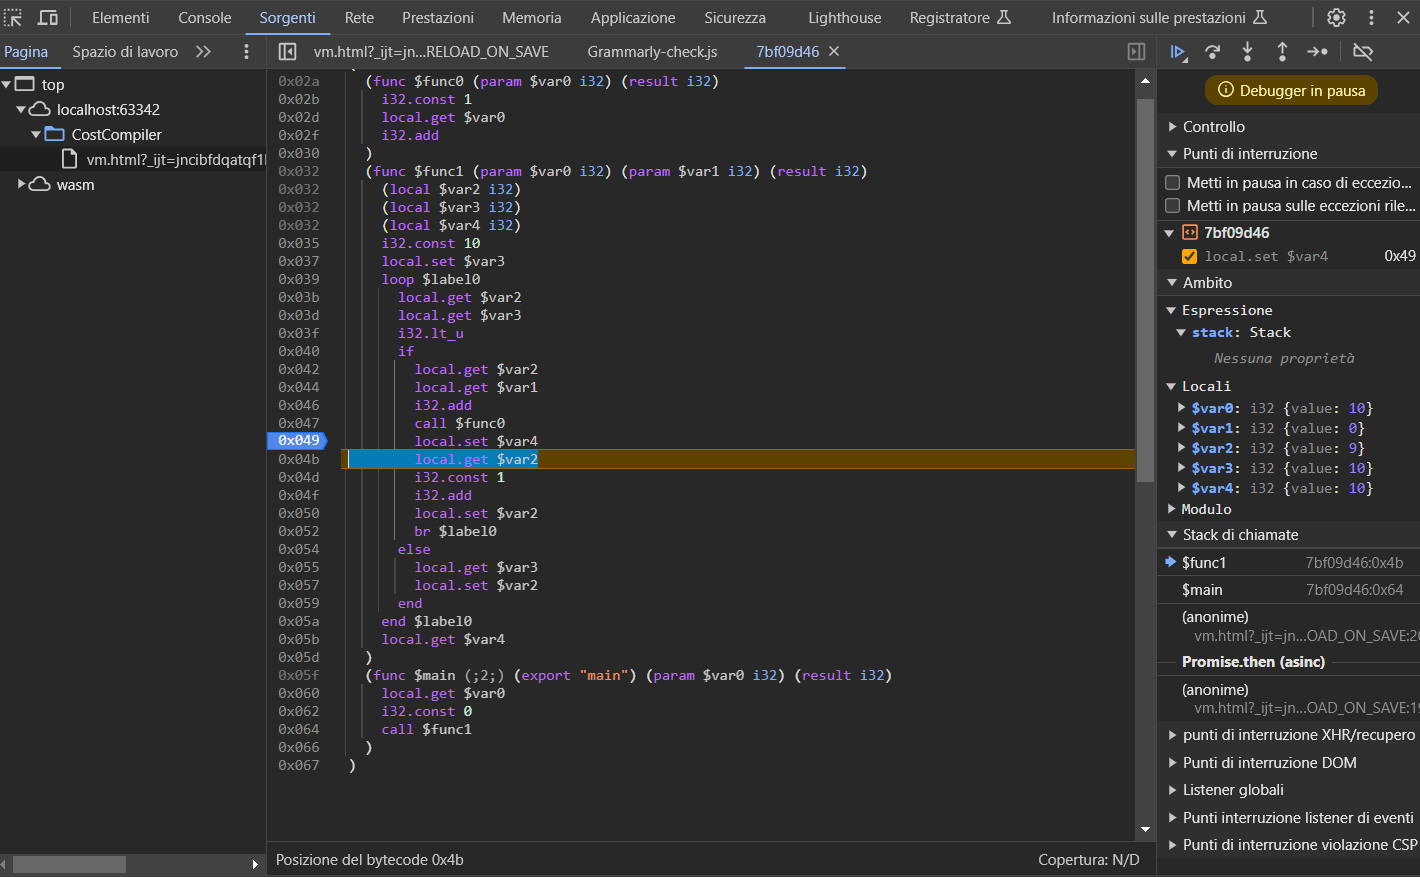
\includegraphics[width=0.8\textwidth]{wasm_debug.png}
    \caption{Debug del file output.wasm}
    \label{fig:wasm_debug}
\end{figure}
Come notiamo il file .wasm é stato caricato correttamente, e possiamo andare a vedere il suo contenuto, inserire breakpoint e andare ad analizzare il runtime del nostro codice.
Notiamo inoltre che il formato WAT a confronto é molto piú leggibile, sopratutto per quanto riguarda il nome delle variabili, Wasm contiene il programma mappando le variabili in $var_0,\dots, var_n$.
A destra troviamo sia lo stack, mentre altre di sotto le variabili che interagiscono in un determinato scope locale, e lo stack di chiamate delle funzioni.

\end{document}